\documentclass[11pt]{article}
\usepackage[sc]{mathpazo} %Like Palatino with extensive math support
\usepackage{fullpage}
\usepackage{amsmath}
\RequirePackage[authoryear,sectionbib,sort]{natbib}
\bibliographystyle{amnatnat}
\linespread{1.7}
\usepackage{graphicx}
\usepackage[utf8]{inputenc}
\usepackage{lineno}
\usepackage{titlesec}
\titleformat{\section}[block]{\Large\bfseries\filcenter}{\thesection}{1em}{}
\titleformat{\subsection}[block]{\Large\itshape\filcenter}{\thesubsection}{1em}{}
\titleformat{\subsubsection}[block]{\large\itshape}{\thesubsubsection}{1em}{}
\titleformat{\paragraph}[runin]{\itshape}{\theparagraph}{1em}{}[. ]\renewcommand{\refname}{Literature Cited}

%%%%%%%%%%%%%%%%%%%%%
% Line numbering
%%%%%%%%%%%%%%%%%%%%%
%
% Please use line numbering with your initial submission and
% subsequent revisions. After acceptance, please turn line numbering
% off by adding percent signs to the lines %\usepackage{lineno} and
% to %\linenumbers{} and %\modulolinenumbers[3] below.
%
% To avoid line numbering being thrown off around math environments,
% the math environments have to be wrapped using
% \begin{linenomath*} and \end{linenomath*}
%
% (Thanks to Vlastimil Krivan for pointing this out to us!)

\title{The Evolutionary Ecology of Individual Foraging Decisions}

% This version of the LaTeX template was last updated on
% November 8, 2019.

%%%%%%%%%%%%%%%%%%%%%
% Authorship
%%%%%%%%%%%%%%%%%%%%%
% Please remove authorship information while your paper is under review,
% unless you wish to waive your anonymity under double-blind review. You
% will need to add this information back in to your final files after
% acceptance.

\author{Pratik R. Gupte$^{1,\ast}$ \\ 
        Christoph F. G. Netz$^{1}$ \\ 
        Franz J. Weissing$^{1}$}

\date{}

\begin{document}

\maketitle

\noindent{} 1. University of Groningen, Groningen 9747AG, The Netherlands.

\noindent{} $\ast$ Corresponding authors; e-mail: p.r.gupte@rug.nl

\bigskip

\textit{Manuscript elements}: EXAMPLE: Figure~1, figure~2, table~1, online appendices~A and B (including figure~A1 and figure~A2). Figure~2 is to print in color.

\bigskip

\textit{Keywords}: Examples, model, template, guidelines.

\bigskip

\textit{Manuscript type}: Article. %Or e-article, note, e-note, natural history miscellany, e-natural history miscellany, comment, reply, invited symposium, or historical perspective.

\bigskip

\noindent{\footnotesize Prepared using the suggested \LaTeX{} template for \textit{Am.\ Nat.}}

\linenumbers{}
\modulolinenumbers[1]

\newpage{}

\section*{Abstract}

% Understanding the causes and consequences of animal movement is key to mechanistically linking individual behaviour with population-level patterns.
% Classical models of individual-to-population foraging distributions do not account for the complex and changeable resource landscapes animals must navigate.
% Neither are the rich behavioural repertoires addressed that animals may exhibit in a foraging context, and their evolution is almost entirely ignored.
% We take a spatially explicit, individual-based simulation approach to model the evolution of individual movement and foraging strategies, and its consequences for population distributions in three simple foraging scenarios of increasing behavioural complexity.
% We show that movement rules and individual foraging strategies co-evolve to optimality in all three scenarios.
% We find that exploitation competition is a relatively weak driver of individual movement and intake, and that this effect depends on the replenishment rate of the resource.
% We also find that when interference competition in the form of kleptoparasitism is allowed, it gives rise to a quasi-predator class of individuals and a third trophic level emerges.
% These quasi-predators compete among themselves much more than they compete with all other individuals, even when they are able to switch from a scrounger to a producer strategy.

\textbf{WORK IN PROGRESS}

\newpage{}

\section*{Introduction}

\textbf{WORK IN PROGRESS}

% The journal does not have numbered sections in the main portion of
% articles. Please refrain from using section references (à la
% section~\ref{section:CountingOwlEggs}), and refer to sections by name
% (e.g. section ``Counting Owl Eggs'').

\section*{Evolutionary Simulation Model of Individual Foraging Decisions}

Our model is an individual-based evolutionary simulation whose most basic components --- the environment size and shape, its gridded structure and each cell's capacity to hold multiple individuals, as well as the discrete conception of time within and between generations --- is taken from Netz et al. \textit{in prep.}.
We conceptualised the model and the scenarios around the behaviour of waders (\textit{Charadrii}, and especially oystercatchers \textit{Haematopus sp.}), which are extensively studied in an optimal foraging context \citep[e.g. ][]{vahl2005, vahl2005a, vahl2005b, ENS1990219}.
We simulated a fixed population with a fixed size of 10,000 individuals moving on a landscape of 512\textsuperscript{2} grid cells, with the landscape wrapped at the boundaries so that individuals passing beyond the bounds at one end re-appear on the diametrically opposite side.
Individuals have a lifetime of $T$ timesteps, with $T$ set to 400 by default.
After their lifetime, individuals reproduce and transmit their heritable traits proportional to their fitness over their lifetime.
The model code (in C++) can be found as part of the Supplementary Material in the Zenodo repository at \textbf{Zenodo/other repository here}.

\subsection*{Flexibility in Foraging Strategies}

Our model considers three main scenarios of flexibility in individual foraging strategies.
The \textbf{first scenario} is an inflexible producer-only case, in which individuals move about on the landscape and probabilistically find and consume discrete prey food items.
Between finding and consuming a food item, individuals must `handle' the prey for a fixed handling time $T_H$ which is constant across prey items.
Prey handling time $T_H$ is set at 5 timesteps by default.
The handling time dynamic is well known from many systems; for instance, it could be the time required for a wader to break through a mussel shell, with the handling action obvious to nearby individuals, and the prey not fully under the control of the finder.
We refer to such individuals as `handlers' for convenience.
Handlers are assumed to be fully absorbed in their processing of prey, and do not make any movements until they have fully handled and consumed their prey.
The \textbf{second scenario} is a fixed-strategy case which adds some flexibility.
Individuals at the start of their lifetime each choose between two foraging strategies, which are then fixed through life.
The strategy choice is based on local environmental cues, and is covered in ``Movement and Foraging Decisions''.
The two strategies are to produce, i.e., to probabilistically find, handle, and consume discrete prey (as in the producer-only case), or to scrounge as a kleptoparasite, i.e., to steal a found prey item from the individual handling it.
We refer to such scroungers as `kleptoparasites' from here onwards.
Kleptoparasites can steal from any handler, regardless of whether that handler acquired its prey by searching or theft.
Kleptoparasites are always successful in stealing from the handler they target; this may be thought of as the benefit of the element of surprise, a common observation in nature.
Having acquired prey, a kleptoparasite need only handle it for $T_H - t_h$ timesteps, where $t_h$ is the time that the prey has already been handled by its previous handler.
The targeted handler deprived of its prey is assumed to flee from the area, and does not make a further movement decision.
Thus kleptoparasites clearly save time on handling compared to a producer, and the time saved increases with the handling time $T_H$ of the prey.
The \textbf{third scenario} is a flexible-strategy case, and individuals are allowed to be plastic in their foraging strategies, and choose between producing and scrounging strategies in each timestep.
Apart from the frequency of the choice, the actual foraging dynamics are the same as described in the fixed-strategy case. Individuals move about on the environment, and each foraging strategy choice is based on local environmental cues (see ``Movement and Foraging Decisions'').

\subsection*{Movement and Foraging Decisions}

Individuals essentially use cues available in timestep $t$ to predict their best move for the next timestep $t+1$, and the strategy associated with that move (when this is allowed).
The movement decision is based on three local environmental cues: (1) the number of discrete prey items $G$, (2) the number of individuals handling  prey $H$ (referred to as `handlers'), and (3) the number of individuals not handling prey $P$ (referred to as `non-handlers').
The notation is chosen in keeping with Netz et al. \textit{in prep.}.
These cues are available to individuals in all three model scenarios.
Individuals occupy a single grid cell on the environment at a time, and assign a suitability score $S$ incorporating $G$, $H$, and $P$ per cell to the nine cells in their Moore neighbourhood (including their current cell).
Following Netz et al. \textit{in prep.}, individuals calculate the cell-specific $S$ as
\begin{linenomath*}
    \begin{equation*}
        S = m_gG + m_hH + m_pP + m_b
    \end{equation*}
\end{linenomath*}
where the weighing factors for each cue $m_g$, $m_h$ and $m_p$, and the bias $m_b$ are genetically encoded and heritable between generations.
Individuals rank their Moore neighbourhood by $S$ in timestep $t$ and move to the highest ranked cell in timestep $t+1$.

Individuals in the producers-only case make no foraging decisions and find food items probabilistically (see ``Prey Environment and Ecological Dynamics'').
In the fixed-strategy case, individuals pick a lifelong foraging strategy in their first timestep ($t_0$), while in the flexible-strategy case, individuals pick a strategy in each timestep $t$ to be deployed in $t+1$.
Individuals in these latter two cases process the cell-specific environmental cues $G$, $H$, and $P$ to determine their foraging strategy $F$ for life (fixed strategy), or in the grid cell into which they have chosen to move in $t+1$ (flexible strategy).
$F$ is determined as
\begin{linenomath*}
    \begin{equation*}
        F = 
    \begin{cases}
        {producer},& \text{if } f_gG + f_hH + f_pP + f_b \geq 0\\
        {scrounger},              & \text{otherwise}
    \end{cases}
    \end{equation*}
\end{linenomath*}
where the cue weights $f_g$, $f_h$ and $f_p$, and the bias $f_b$ are also genetically encoded and heritable between generations.

In both latter cases that allow for kleptoparasitism, individuals make their foraging strategy choice for the next timestep after they have passed through the ecological dynamics of their current location.
This excludes individuals that have been stolen from are an important exception; these fleeing agents are moved to a random cell within a Chebyshev distance of 5, and do not make a foraging decision there.
Thus kleptoparasitism not only gains individuals prey items while depriving the targeted individual, it also displaces a potential competitor.
All individuals move simultaneously, and attempt to implement the foraging strategy chosen for their new location (see below).

\subsection*{Prey Environment and Ecological Dynamics}

Since our model was initially conceived to represent foraging waders, we developed a resource landscape based on mussels (family \textit{Mytilidae}) that are commonly found in inter-tidal systems.
Mussels beds share some important characteristics with other discrete prey items.
Firstly, mussels are immobile relative to their consumers, and their abundances are largely driven by extrinsic environmental gradients and very small-scale interactions \citep{dejager2020, dejager2011}.
Secondly, in common with many ecological systems \citep{levin1992}, mussels are not uniformly distributed across the inter-tidal mudflats, and are instead strongly spatially patterned into clusters (`beds') \citep{dejager2020, dejager2011}.
Thirdly, while prey or their signs in an area are often visible to consumers, consumers are not always certain of obtaining one of these prey, since prey can show small-scale anti-predator avoidance responses.

We captured these essential aspects of prey dynamics when implementing the resource landscape on which our individuals move.
We modelled relative prey immobility and extrinsically driven abundance by assigning each grid cell of the resource landscape a constant probability of generating a new prey item per timestep, which we refer to as the growth rate $r$.
We modelled clustering in the abundance of prey by having the distribution of $r$ across the grid cells take the form of 1,024 uniformly distributed resource peaks with $r$ declining from the centre of each peak to its periphery (Figure X).
Effectively, the cell at the centre of each patch generates a prey item five times more frequently than the cells at the edges.
Thus for a simulation-specific baseline $r_{base}$ = 0.03, the central cell of a resource peak  would have an $r_{centre} = 0.03$, and generate 3 items every 100 timesteps, compared with $r_{edge} = 0.006$, or 0.6 items generated in 100 timesteps.
We ran the simulation with $r_{base}$ values of 0.001, 0.01, 0.03, and 0.05, which we considered a sufficiently broad range. 
Cells in our landscape were modelled as being able to hold a maximum of $K$ prey items, with the default $K$ = 5.
While a cell is at carrying capacity its $r$ is 0.
We modelled near-perfect intermediate-range perception but uncertain short-range acquisition of prey by allowing individuals to perceive all prey items $G$ in a cell, but giving individuals which choose a producer strategy only a probability of finding one of these prey.
The probability of finding a prey item $p(success)$ is given as the probability of not finding any of $G$ prey
\begin{linenomath*}
    \begin{equation*}
        p({success}) = 1 - \left(1 - p_i\right) ^ G
    \end{equation*}
\end{linenomath*}
where $p_i$ is the detection probability of each of $G$ items, which is uniformly set to 0.2 by default for all items.

Since we model foraging events as occurring simultaneously, it is possible for more producers to be considered successful in finding prey than there are discrete items in that cell.
We resolve this simple case of exploitation competition by assigning $G$ prey among some $N$ successful finders at random.
Producers that are assigned a prey item in timestep $t$ begin handling it, and are considered to be handlers for the purposes of timestep $t+1$ (primarily movement and foraging decisions of other individuals).
It is important to note that a producer that has converted into a handler in timestep $t$ is not an available target for kleptoparasites until timestep $t+1$.
Producers that are not assigned a prey item are considered idle during timestep $t$, and are counted as non-handlers for $t+1$.

Kleptoparasites in the fixed- or flexible-strategy case face a slightly different challenge.
All kleptoparasites in a cell successfully steal from a handler, contingent on the number of handlers matching or exceeding the number of kleptoparasites in timestep $t$.
When the number of kleptoparasites exceeds handlers, handlers are assigned among kleptoparasites at random.
Successful kleptoparasites convert into handlers, and similar to producer-handlers are unavailable as targets to other kleptoparasites until the next timestep.
Unsuccessful kleptoparasites are considered idle, and are also counted as non-handlers for timestep $t+1$.
A handler that finishes processing its prey in timestep $t$ returns to the non-handler state and is assessed as such by other agents when determining movements for $t+1$.

Individuals move and forage on the resource landscape for $T$ timesteps per generation, and $T$ is set at 400 by default.
Handling a food item requires a maximum of $T_H$ timesteps, during which the handler is immobile.

\subsection*{Reproduction and the Evolution of Decision Making}

At the end of each generation, the population is replaced by its offspring, maintaining the fixed population size, and the decision-making weights which determine individual movement ($m_g$, $m_h$, $m_p$, $m_b$) and foraging strategy choice ($f_g$, $f_h$, $f_p$, $f_b$) are transmitted from parent individuals to offspring.
The number of offspring of each parent is proportional to the parent's share of the population fitness, and this is implemented as a weighted lottery that selects a parent for each offspring.
The total lifetime intake of individuals is used as a proxy of fitness, and the population's total fitness is its total intake.
The decision-making weights are subject to independent random mutations with a probability of 0.001.
The size of the mutation (either positive or negative) is drawn from a Cauchy distribution with a scale of 0.01 centred on the current value of the weight to be mutated.
This allows for a small number of very large mutations while the majority of mutations are small.
Autocorrelation in the landscape coupled with limited natal dispersal can lead to spatial heterogeneity becoming fixed in populations, as lineages adapt to local conditions.
Among other things, this could lead to population-level movements due to differential reproduction that mirror shifts in resource abundance, rather than individual movement.
To ensure individual movement rules evolved, we intialised each offspring at a random location on the landscape, and also reset its total intake to zero.

\subsection*{Simulation Output and Analysis}

\paragraph{Spatial Distribution of Individuals, their Intake, and Prey Items}

Over each of the last eight generations of the simulation (991 -- 998), we summed the following for each grid cell $ij$ over the generation's timesteps: (1) the number of prey items $G$, (2) the number of individuals following each of the two strategies, producer $N_p$ or kleptoparasitic scrounger $N_s$, and (3) the intake (in food items consumed after handling) by agents following each of the two strategies, producer $I_p$ or kleptoparasite $I_s$.
For instance, the number of producer individuals in a generation to inhabit a cell $ij$ would be
\begin{linenomath*}
    \begin{equation*}
        N_p = \sum_{t=0}^{i=T} n_{p_t}
    \end{equation*}
\end{linenomath*}
where $t \in (0, 1 \dots T = 400)$, and $n_{p_t}$ is the number of producers in cell $ij$ at each timestep $t$.
We saved this generation- and simulation- specific data to file, and these data are available at the Zenodo/IRODS repository at \textbf{Zenodo/other link here}.
The volume of data at this stage was comparable to a very high-resolution, long-term ecological study, and we handled it accordingly.
First, we processed the data to get the timestep-averaged values of $G$, $N_p$, $N_s$, $I_p$, and $I_s$ for each cell, dividing each value by $T$ (400).
From this data, we calculated the per-capita intake rate ($I$ per $t$) on each cell for each of the two strategies separately, which we denote as $R_p$ (producers) and $R_s$ (scroungers).
% The total intake rate $R$ per cell was then $R_p + R_s$.
We plotted the timestep- and generation-averaged item count ($G$), strategy count ($N_p$, $N_s$), and absolute and per-capita intake ($I_p$, $I_s$, and $R_p$, $R_s$) in relation to grid-cell quality (the growth rate, $r$) to investigate the spatial distribution of individuals (see Figure X).

\paragraph{Generalised Functional Response}

In our simulation, individuals perceive and respond to the standing stock of prey items $G$ on a cell rather than its growth rate $r$.
This standing stock is unpredictable due to consumption by other individuals.
To understand the consequences of movement, we need to investigate how individual intake rate varies with $G$ as well as the presence of potential competitors.
Thus we examined the generalised functional response ($W$) \textit{sensu}\citet{meer1997}.
We plotted the per-capita intake rate achieved by individuals on grid-cells with similar numbers of prey items ($G$) and individuals ($N_p + N_s$) (see Figure Xa).
We did this separately for $W_p$ and $W_s$, the generalised functional response of individuals using the producer and kleptoparasitic scrounger respectively (see Figure Xb, Xc).
We modelled the effect of competition and resource availability on $W_p$ and $W_s$ using a simple generalised linear model (GLM) with either $W_p$ or $W_s$ as the response, and the number of individuals and the number of prey items as the only additive predictors.
We repeated this for simulations with different baseline growth rates $r$, and examined variation in the contribution of competition and resource availability in the \textbf{form of the linear model coefficients of individual density and item density, respectively (see Figure X)}.
These linear models took the form
\begin{linenomath*}
    \begin{equation*}
        W = \beta_0 + \beta_1 G + \beta_2 (N_p + N_s)
    \end{equation*}
\end{linenomath*}
where $W$ is either $W_p$ or $W_s$.
We fit these models for each $r_{base}$ separately, but did not distinguish between replicates.

\paragraph{Decision Making Weights}

To understand the evolutionary consequences of our simulation, we exported the the decision-making weights which determine individual movement ($m_g$, $m_h$, $m_p$, $m_b$) and foraging strategy choice ($f_g$, $f_h$, $f_p$, $f_b$) of each individual in every generation of the simulation.
We examined how the frequency of these weights changed over the simulation, i.e., how the weights evolved.
We visualised weights' evolution after scaling them between -1 and +1 using a hyperbolic tangent function, and binning the scaled values into intervals of 0.1.
We refer to these scaled and binned values as phenotypes for convenience.
Weights at or near -1 would represent the maximum evolved avoidance of an environmental cue (in relation to a movement weight) or the greatest evolved negative effect of a cue on choosing the foraging strategy (in relation to a strategy choice weight).
Similarly, weights at or near +1 represent the greatest evovled preference for or positive effect of a cue on the movement and strategy choice mechanism of an individual.

\section*{Simulation Model Outcomes}

\subsection*{Emergence of a Dynamic Equilibrium}

\textbf{WORK IN PROGRESS}

\subsection*{Evolution of Movement Decisions}

\paragraph*{Response to Prey Items}

Populations across scenarios consistently evolved to move towards food items, with all individuals evolving positive values of $m_g$ across regrowth rates (Fig. 1.a).
However, across scenarios, replicates and growth rates, populations did not converge upon a single value of $m_g$, with a similar number of phenotypes evolved across replicates (Fig. 1.e).
Scenarios 2 and 3 showed opposite relationships between the number of $m_g$ phenotypes and $r_{base}$: in scenario 2, there were only about half as many phenotypes as in scenario 3 for $r_{base} \leq$ 0.1, while at the highest $r_{base}$ (0.25), there were almost four times as many phenotypes in scenario 2 as in scenario 3.

\paragraph*{Response to Handling Individuals}

Populations across scenarios evolved to move towards handling individuals at low growth rates, with most individuals in the final generation having positive values of $m_h$ ($r_{base} <$ 0.05; Fig. 1.b).
At higher growth rates, populations in scenario 3 consistently evolved a preference for handling individuals, with variation in the number of phenotypes declining with increasing $r_{base} $(Fig. 1.b, f).
In scenarios 1 and 2 however, the proportion of the population with an evolved preference for moving towards handling individuals declined at higher growth rates, with only between 25\% and 50\% of the population showing such a preference at the highest growth rate.
This decreasing preference for handlers was accompanied by an increase in the number of negative phenotypes of $m_h$, though the number of positive phenotypes was maintained despite the lower proportion of individuals with a positive $m_h$.

\paragraph{Response to Non-Handling Individuals}

Acros scenarios, populations evolved to move away from non-handling individuals when growth rates were low, with most individuals in the final generation having negative values of $m_p$ ($r_{base} <$ 0.1; Fig. 1.c).
At higher growth rates, however, populations in scenarios 1 and 2 evolved no particular preference or avoidance of non-handlers, while in scenario 3 the population consistently evolved to move towards non-handling individuals.
There was wide variation in the strength of avoidance (and at higher $r_{base}$, preference), with multiple $m_p$ phenotypes (Fig. 1.g).

\paragraph*{Overall Response to Individuals}

On summing, transforming, and binning the weights for handling and non-handling individuals, the evolved preferences for individuals in total were distinct to each scenario.
Populations in scenario 3 evolved a consistent preference for moving towards individuals overall (Fig. 1.d).In scenario 2, the proportion of the population with an overall preference for moving towards individuals declined linearly with growth rate.
At the two highest growth rates (0.1, 0.25), about 50\% of fixed-strategy individuals preferred to move towards other individuals.
Scenario 1 showed a strongly non-linear, inverse hump-shaped relationship between the preference for individuals and growth rates.
At very low growth rates ($r_{base} \approx$ 0.001), about half the population had an overall preference for moving towards other individuals.
This proportion declined until nearly all individuals avoided each other when choosing where to move for  0.01 $\geq r_{base} <$ 0.1.
Across high growth rates ($\geq$ 0.1), an increasing proportion of individuals preferred to move towards other individuals overall (Fig. 2.d).

\begin{figure*}[h]
    \centering
    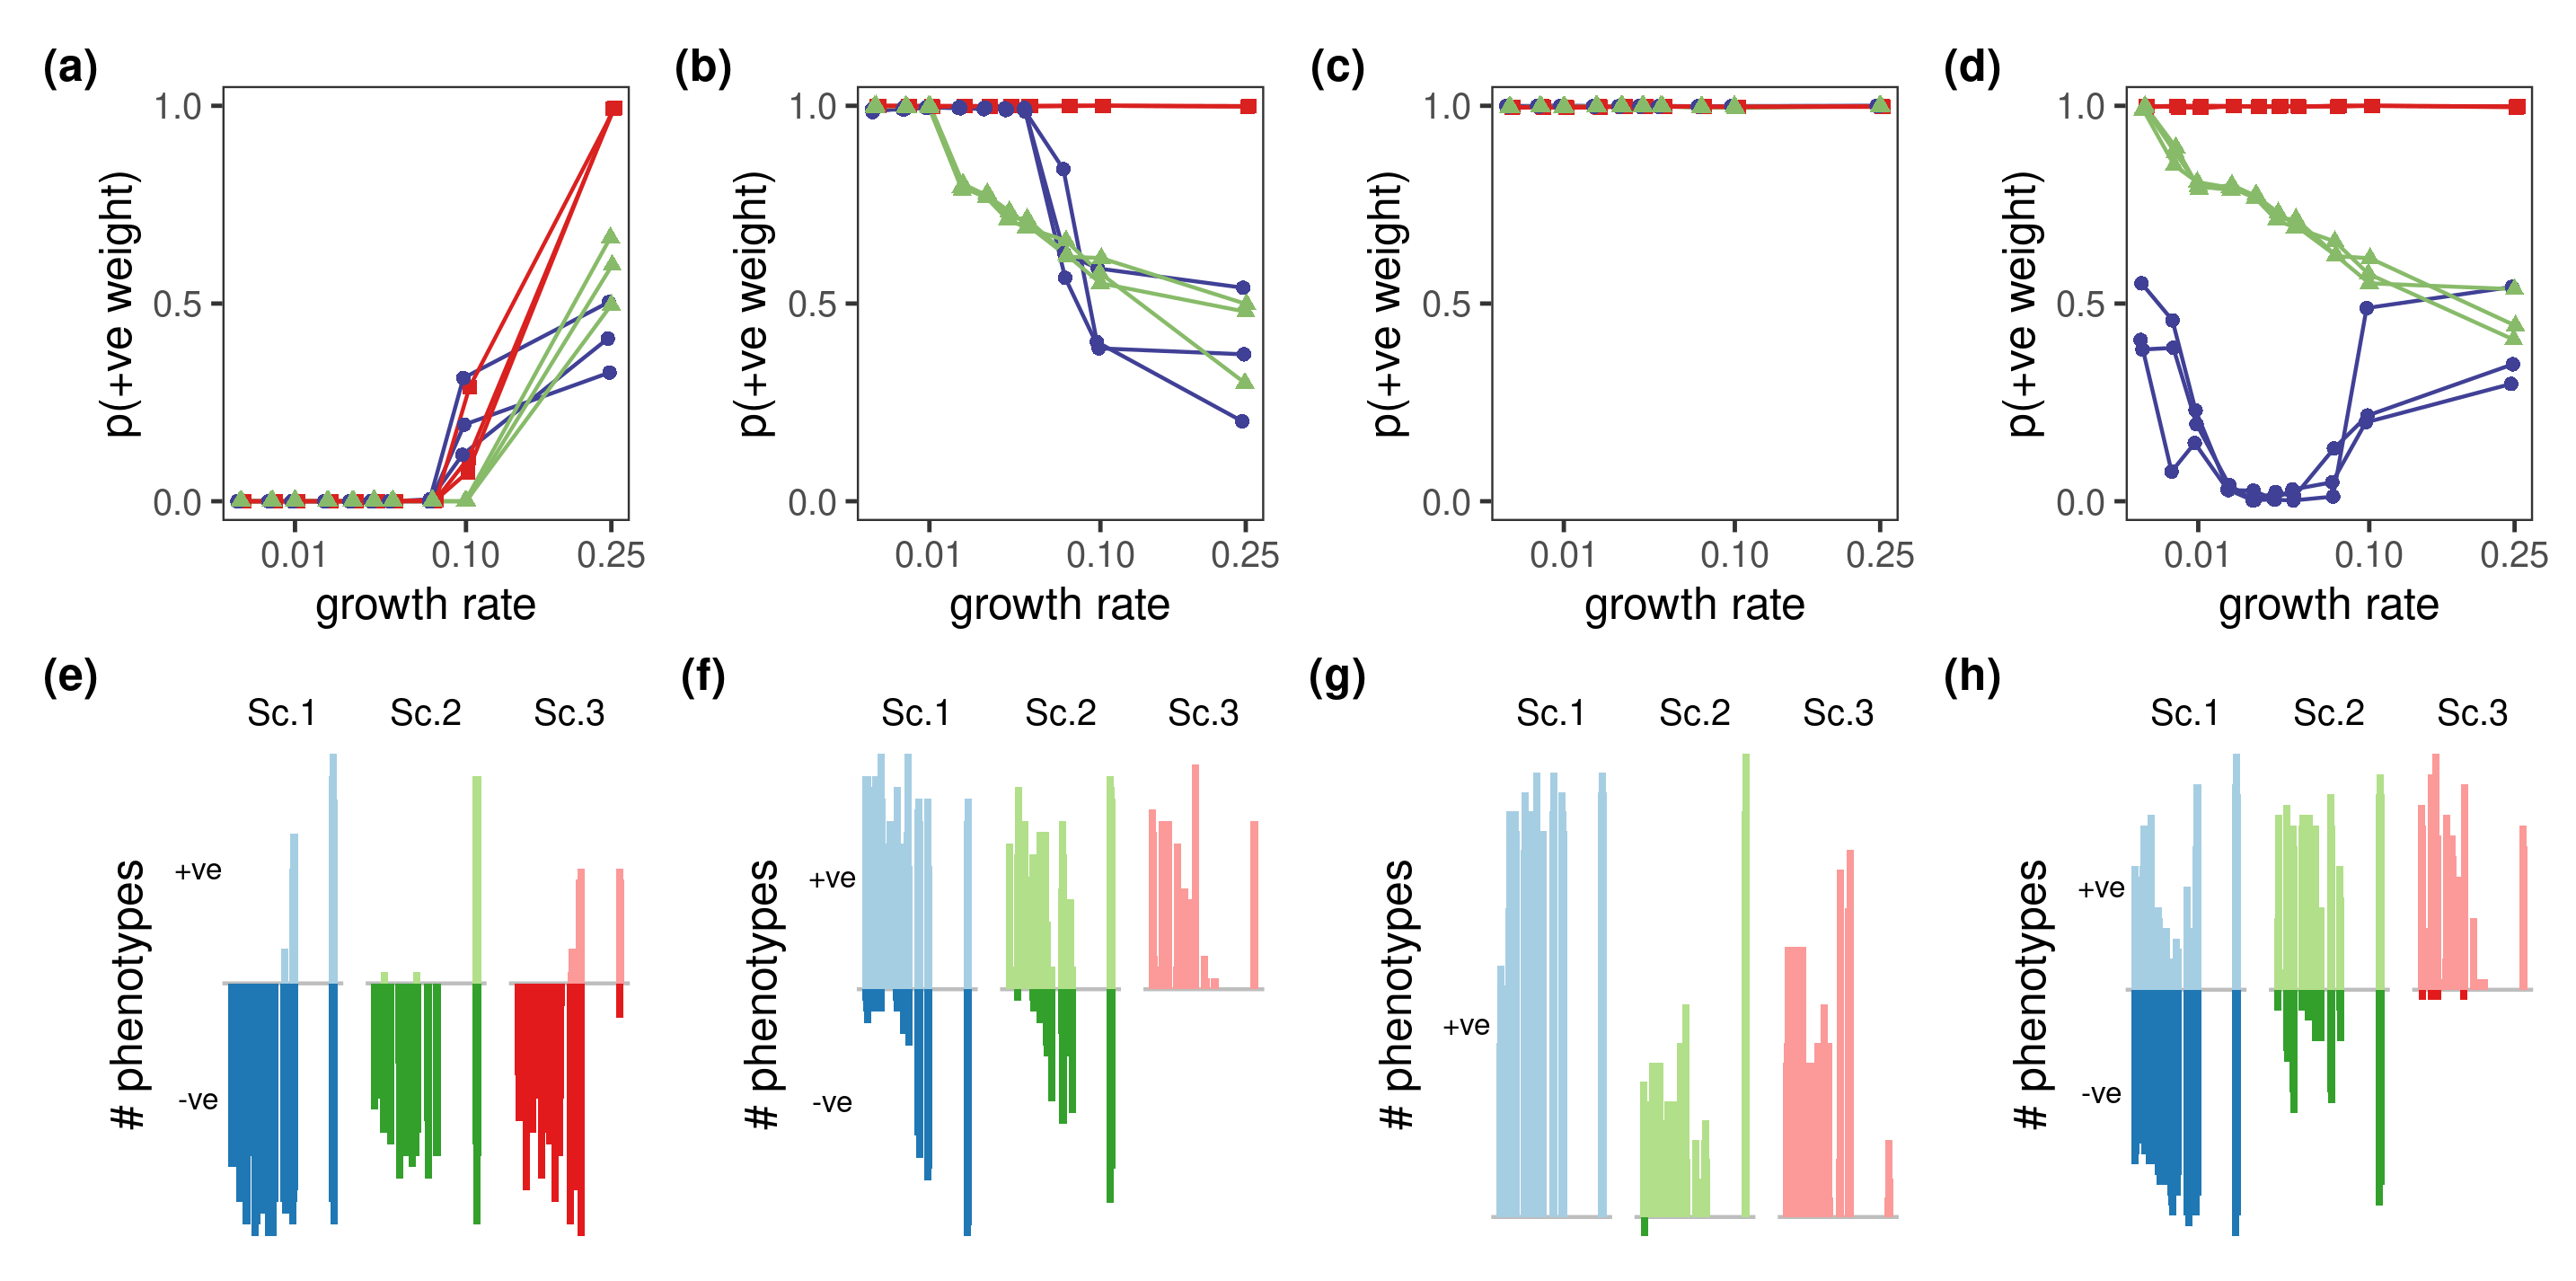
\includegraphics[width=0.99\textwidth]{figures/fig_03_move_weight_end_vals.png}
    \caption{
        Proportion of individuals in populations evolved across different regrowth rates selecting \textit{for} environmental cues in deciding movement.
        Panels \textbf{(a -- d)} show the proportion of individuals with positive weights for each cue: \textbf{(a)} non-handling individuals, \textbf{(b)} handling individuals, \textbf{(c)} prey items, and \textbf{(d)} individuals overall.
        Colours and shapes represent scenarios (blue circles: \textit{producers-only}; green triangles: \textit{fixed-strategy}; red squares: \textit{flexible-strategy}).
        While lines connect similarly numbered replicates across $r_{base}$, these are entirely independent simulations.
        %%
        Panels \textbf{(e -- h)} show the number of distinct values for each weight in the population in panels \textbf{(a -- d)} separated by the sign (positive or negative): \textbf{(e)} non-handling individuals, \textbf{(f)} handling individuals, \textbf{(g)} prey items, and \textbf{(h)} individuals overall.
        Bar colours represent scenarios (blue: \textit{producers-only}; green: \textit{fixed-strategy}; red: \textit{flexible-strategy}), while the hue represents the sign (light: positive, dark: negative).
        %%
        Individuals avoid non-handlers for $r_{base} \leq$ 0.1, after which they evolve neutrally in scenarios 1 and 2, and strongly positive values in scenario 3  (\textbf{a, e}).
        Similarly, most individuals in scenarios 1 and 2 move towards handlers, but the proportion and diversity of negative weights increases at $r_{base} \geq$ 0.1 (\textbf{b, f}). Individuals in scenario 3 consistently move towards handlers, and individuals overall (\textbf{b, f, d, h}).
        Overall, in scenario 1 individual preference for moving towards other individuals has an inverse-humped relationship with $r_{base}$, while in scenario 2 it shows a steady linear decline.
    }
    \label{fig:figure_pipeline}
\end{figure*}

\subsection*{Evolution of Foraging Strategy}

Populations in scenario 3 were fixed to choose a producer strategy, and their foraging strategy weights evolved neutrally, providing a null model of weight evolution against which to compare scenarios 2 and 3.
Populations in scenario 3 did not show a consistently evolved bias towards choosing a producing strategy, with no discernible pattern in the proportion of the population bearing a positive $f_b$ (Fig. 2. a).
However, populations in scenario 2 showed an increasing proportion of individuals biased towards a foraging strategy with increasing $r_{base}$.
At the highest growth rate, all evolved individuals in scenario 3 were biased towards producing (Fig. 2.a).

Populations across scenarios, growth rates, and replicates evolved to seemingly ignore prey items and non-handling individuals when making a foraging decision, with no consistency in the proportion of individuals bearing positive $f_g$ and $f_p$ across replicates of the same scenario and growth rate(Fig. 2.b,d).
Howevever, evolved populations in scenario 3 were more likely to uniformly choose a foraging strategy based on the number of non-handling individuals, with more variation within rather than between growth rates.

The number of handling individuals was not processed similarly by individuals evolved in scenario 2 when choosing a strategy, with proportions oscillating around 0.5 (Fig. 2.c).
In scenario 3, populations consistently evolved to choose a kleptoparasitic-scrounger strategy in the presence of handlers (Fig. 2c.).
This proportion was reduced at very low growth rates ($r_{base} <$ 0.01; Fig. 2.c).

\begin{figure*}[h]
    \centering
    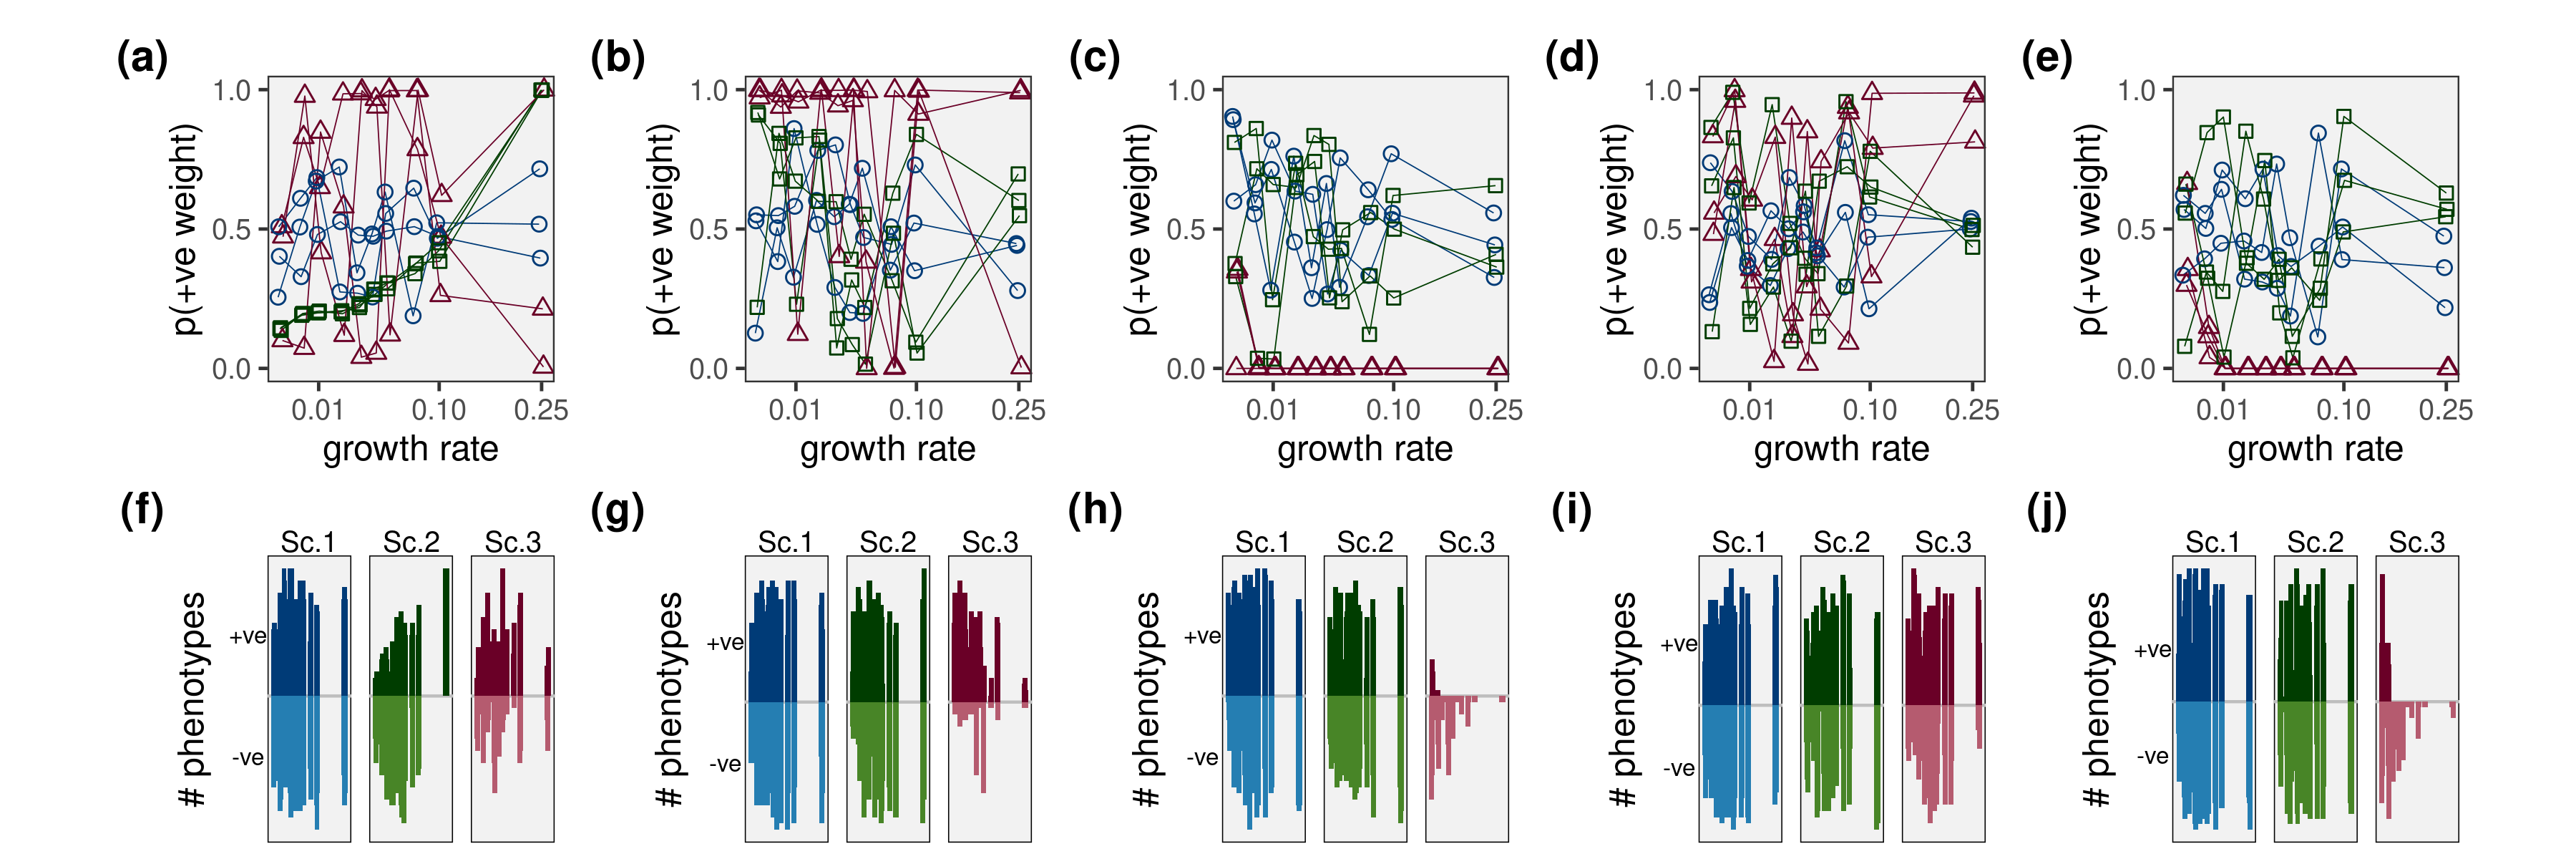
\includegraphics[width=0.99\textwidth]{figures/fig_04_strategy_weight_end_vals.png}
    \caption{
        The proportion of individuals choosing a foraging strategy based on environmental cues is not linked to the regrowth rate.
        Panels \textbf{(a -- e)} show the proportion of individuals with positive weights for each cue: \textbf{(a)} bias, \textbf{(b)} non-handling individuals, \textbf{(c)} handling individuals, \textbf{(d)} prey items, and \textbf{(e)} all cues combined.
        Colours and shapes represent scenarios (blue circles: \textit{producers-only}; green triangles: \textit{fixed-strategy}; red squares: \textit{flexible-strategy}).
        Lines connect similarly numbered replicates across $r_{base}$, but these are entirely independent simulations.
        %%
        Panels \textbf{(f -- j)} show the number of distinct values for each weight in the population in panels \textbf{(a -- e)} separated by the sign (positive or negative): \textbf{(f)} bias, \textbf{(g)} non-handling individuals, \textbf{(h)} handling individuals, \textbf{(i)} prey items, and \textbf{(j)} all cues combined.
        Bar colours represent scenarios (blue: \textit{producers-only}; green: \textit{fixed-strategy}; red: \textit{flexible-strategy}), while the hue represents the sign (light: positive, dark: negative).
        %%
        Individuals' weights in scenario 1 evolve neutrally since they are only allowed a producer strategy.
        However, scenario 2 also results in neutral evolution of all weights except $f_b$, with a larger proportion of individuals biased towards producing at high $r_{base}$.
        Almost all individuals in scenario 3 choose to steal except at very low $r_{base}$, with $f_h$ the strongest contributor to the decision.
    }
    \label{fig:figure_pipeline}
\end{figure*}

\subsection*{Spatial Distribution of Individuals and Prey}

\paragraph{Individual Distributions}

There number of individuals on a cell increased with its growth rate $r$, but there was substantial variation across cells with the same $r$. 
This variation was larger with increasing $r$ since there were fewer cells with higher $r$.
In the producer-only case, individual abundance showed a linear increase with cell quality, with the slope increasing with the simulation growth rate $r_{base}$.
%%
When two strategies were allowed however, there were strong differences in how they were distributed across cell qualities.
In the fixed-strategy case, the abundance of producer individuals was uniformly low across cell qualities, while the abundance of scrounging kleptoparasites had a sigmoidal relationship with quality, mediated by $r_{base}$.
In the flexible-strategy case, the use of either strategy was nearly invariant with cell quality.
At very low $r_{base}$ (0.001) the kleptoparasitic strategy was more ofen used than the producer strategy, while at higher $r_{base}$, the producer strategy was more common across cell quality.

\paragraph{Consequences for Prey Item Distribution}

The distributon of items $G$ varied considerably between scenarios and simulation-specific baseline growth rates $r_{base}$.
In the \textbf{first scenario} $G$ was insensitive to $r$, and items were uniformly distributed across cells of different growth rates.
$G$ was not signficantly different among simulations with different $r_{base}$.
In the \textbf{second scenario} $G$ increased strongly with $r$, and the curve of $G ~ r$ varied with $r_{base}$.
The $G ~ r$ transformed from roughly linear ($r_{base}$ = 0.001), to exponential ($r_{base}$ = 0.01), and finally to sigmoidal ($r_{base} \in$ 0.03, 0.05) [see Figure X].
In the \textbf{third scenario} $G$ varied only weakly across cells with different $r$, and the $G ~ r$ response had a positive slope only for the highest $r_{base}$ of 0.03 and 0.05.

\subsection*{Generalised Functional Response}

The model coefficients of $G$ and $N_p + N_s$ changed non-linearly in relation to $r_{base}$ (Figure X).
%%
In the producers-only case, the coefficient $\beta_2$ increased with $r_{base}$ when $r_{base} \leq$ 0.03, after which it decreased below zero for $r_{base}$ = 0.25.
Similarly, the coefficient of items $\beta_1$ was highest at $r_{base}$ = 0.03, decreasing to zero for $r_{base}$ = 0.1 and 0.25.
%%
In the fixed-strategy case, $\beta_1$ (items) was at or near zero across all $r_{base}$.
However, $\beta_2$ for both $W_p$ and $W_s$ was near zero for $r_{base} \leq$ 0.05, positive for $r_{base} \in 0.075, 0.1$, and zero for $r_{base}$ = 0.25.
%%
In the flexible-strategy case, both $\beta_1$ and $\beta_2$ showed a hump-shaped relationship with $r_{base}$ for both $W_p$ and $W_s$, with the highest values at intermediate growth rates.

% If you have deposited data to Dryad, you should cite them somewhere in the main text (usually in the Methods or Results sections). A sentence like the following will do. All data are available in the Dryad Digital Repository (\citealt{CookEtAl2015}).

\section*{Discussion}

\section*{Conclusion}


%%%%%%%%%%%%%%%%%%%%%
% Acknowledgments
%%%%%%%%%%%%%%%%%%%%%
% You may wish to remove the Acknowledgments section while your paper 
% is under review (unless you wish to waive your anonymity under
% double-blind review) if the Acknowledgments reveal your identity.
% If you remove this section, you will need to add it back in to your
% final files after acceptance.

\section*{Acknowledgments}

The authors thank Hanno Hildenbrandt for contributing to the coding of the simulation model \textit{Kleptomove}; 
Matteo Pederboni for contributing to the initial stages of the simulation model; 
and members of the Modelling Adaptive Response Mechanisms Group and of the Theoretical Biology department at the University of Groningen for helpful discussions on the manuscript.

\bibliography{kleptomove}

\newpage{}

\section*{Appendix A: Supplementary Figures}

% In many cases, The American Naturalist allows authors to typeset 
% their own supplementary material in an author-supplied PDF. For author-
% supplied PDFs, please consult the AmNat_supp_template.tex document,
% available from https://www.journals.uchicago.edu/journals/an/instruct 
%
% By contrast, the Appendix instructions below apply to cases in which
% supplementary material is to be typeset by the AmNat editorial staff.
% That notably includes descriptions of methods, tables defining parameters,
% and other material necessary for reproducing the MS's results.
%
% Please reset counters for the appendix (thus normally figure A1, 
% figure A2, table A1, etc.).
%
% In certain cases, it may be appropriate to have a PRINT appendix in
% addition to (or instead of) an online appendix. In this case, please 
% name the print appendix Appendix A, and any subsequent appendixes (if 
% there are any) should be named Online Appendix B, Online Appendix C,
% etc.
%
% Counters for each appendix should match the letter of that appendix.
% For example, tables in Appendix C should be numbered table C1, table C2,
% etc. This applies to tables, equations, and figures.
%
% It's better not to use the \appendix command, because we have some
% formatting peculiarities that \appendix conflicts with.

\renewcommand{\theequation}{A\arabic{equation}}
% redefine the command that creates the equation number.
\renewcommand{\thetable}{A\arabic{table}}
\setcounter{equation}{0}  % reset counter 
\setcounter{figure}{0}
\setcounter{table}{0}

\subsection*{Fox--dog encounters through the ages}

% The quick red fox jumps over the lazy brown dog. The quick red fox has always jumped over the lazy brown dog. The quick red fox began jumping over the lazy brown dog in the 19th century and has never ceased from so jumping, as we shall see in figure~\ref{Fig:Jumps}. But there can be surprises (figure~\ref{Fig:JumpsOk}).

% If the order and location of figures is not otherwise clear, feel free to include explanatory dummy text like this:

% [Figure A1 goes here.]

% [Figure A2 goes here.]

% \subsection*{Further insights}

% Tables in the appendices can appear in the appendix text (see table~\ref{Table:Rivers} for an example), unlike appendix figure legends which should be grouped at the end of the document together with the other figure legends.

% \begin{table}[h]
% \caption{Various rivers, cities, and animals}
% \label{Table:Rivers}
% \centering
% \begin{tabular}{lll}\hline
% River        & City        & Animal            \\ \hline
% Chicago      & Chicago     & Raccoon           \\
% Des Plaines  & Joliet      & Coyote            \\
% Illinois     & Peoria      & Cardinal          \\
% Kankakee     & Bourbonnais & White-tailed deer \\
% Mississippi  & Galena      & Bald eagle        \\ \hline
% \end{tabular}
% \bigskip{}
% \\
% {\footnotesize Note: See table~\ref{Table:Founders} below for further table formatting hints.}
% \end{table}

% Lorem ipsum dolor sit amet, as we have seen in figures~\ref{Fig:Jumps} and \ref{Fig:JumpsOk}.

\newpage{}
\renewcommand{\theequation}{B\arabic{equation}}
% redefine the command that creates the equation number.
\renewcommand{\thetable}{B\arabic{table}}
\setcounter{equation}{0}  % reset counter 
\setcounter{table}{0}

\section*{Appendix B: Additional Methods}

\subsection*{Measuring the height of fox jumps without a meterstick}

% Pellentesque ac nibh placerat, luctus lectus non, elementum mauris. 
% Morbi odio velit, eleifend ut hendrerit vitae, consequat sit amet 
% nulla. Pellentesque porttitor vitae nisl quis tempus. Pellentesque 
% habitant morbi tristique senectus et netus et malesuada fames ac 
% turpis egestas. Praesent ut nisi odio. Vivamus vel lorem gravida 
% odio molestie volutpat condimentum et arcu (\citealt{tytler-mqos}). 

% \begin{equation}
% { \frac{1}{N_k-1} \sum \limits_{t=1}^{N_k} (M_{tjk} - \bar{M}_{jk})^2}
% \end{equation}

% \subsection*{Quantifying the brownness of the dog}

% Pellentesque eu nulla odio (\citealt{Xiao2015,CookEtAl2015}). Nulla aliquam porta metus, quis malesuada orci faucibus quis. Suspendisse nunc magna, tristique sit amet sollicitudin nec, elementum et lacus. Sed vitae elementum mi. In hac habitasse platea dictumst. Etiam eu tortor elit. Sed ac tortor purus. Aliquam volutpat, odio sit amet posuere pretium, dolor ex interdum ante, sed luctus quam eros ac nulla. 

% \begin{equation}
% { (\sum \limits_{p=1}^P {n_{sp}})^{-1}\sum \limits_{p=1}^P {n_{sp}Q_{p}}}
% \end{equation}

\newpage{}

%%%%%%%%%%%%%%%%%%%%%
% Bibliography
%%%%%%%%%%%%%%%%%%%%%
% You can either type your references following the examples below, or
% compile your BiBTeX database and paste the contents of your .bbl file
% here. The amnatnat.bst style file should work for this---but please
% let us know if you run into any hitches with it!
%
% If you upload a .bib file with your submission, please upload the .bbl
% file as well; this will be required for typesetting.
%
% The list below includes sample journal articles, book chapters, and
% Dryad references.

\newpage{}

\section*{Tables}
\renewcommand{\thetable}{\arabic{table}}
\setcounter{table}{0}

% \begin{table}[h]
% \caption{Founders of \textit{The~American Naturalist}}
% \label{Table:Founders}
% \centering
% \begin{tabular}{lll}\hline
% Early editor            & Years with the journal \\ \hline
% Alpheus S. Packard Jr.  & 1867--1886 \\
% Frederick W. Putnam     & 1867--1874 \\ 
% Edward S. Morse         & 1867--1871 \\ 
% Alpheus Hyatt           & 1867--1871 \\
% Edward Drinker Cope$^a$ & 1878--1897 \\
% J.~S. Kingsley          & 1887--1896 \\ \hline 
% \end{tabular}
% \bigskip{}
% \\
% {\footnotesize Note: Table titles should be short. Further details should go in a `notes' area after the tabular environment, like this. $^a$ Published the first description of \textit{Dimetrodon}.}
% \end{table}

\newpage{}

\section*{Figure legends}

% \begin{figure}[h!]
% % 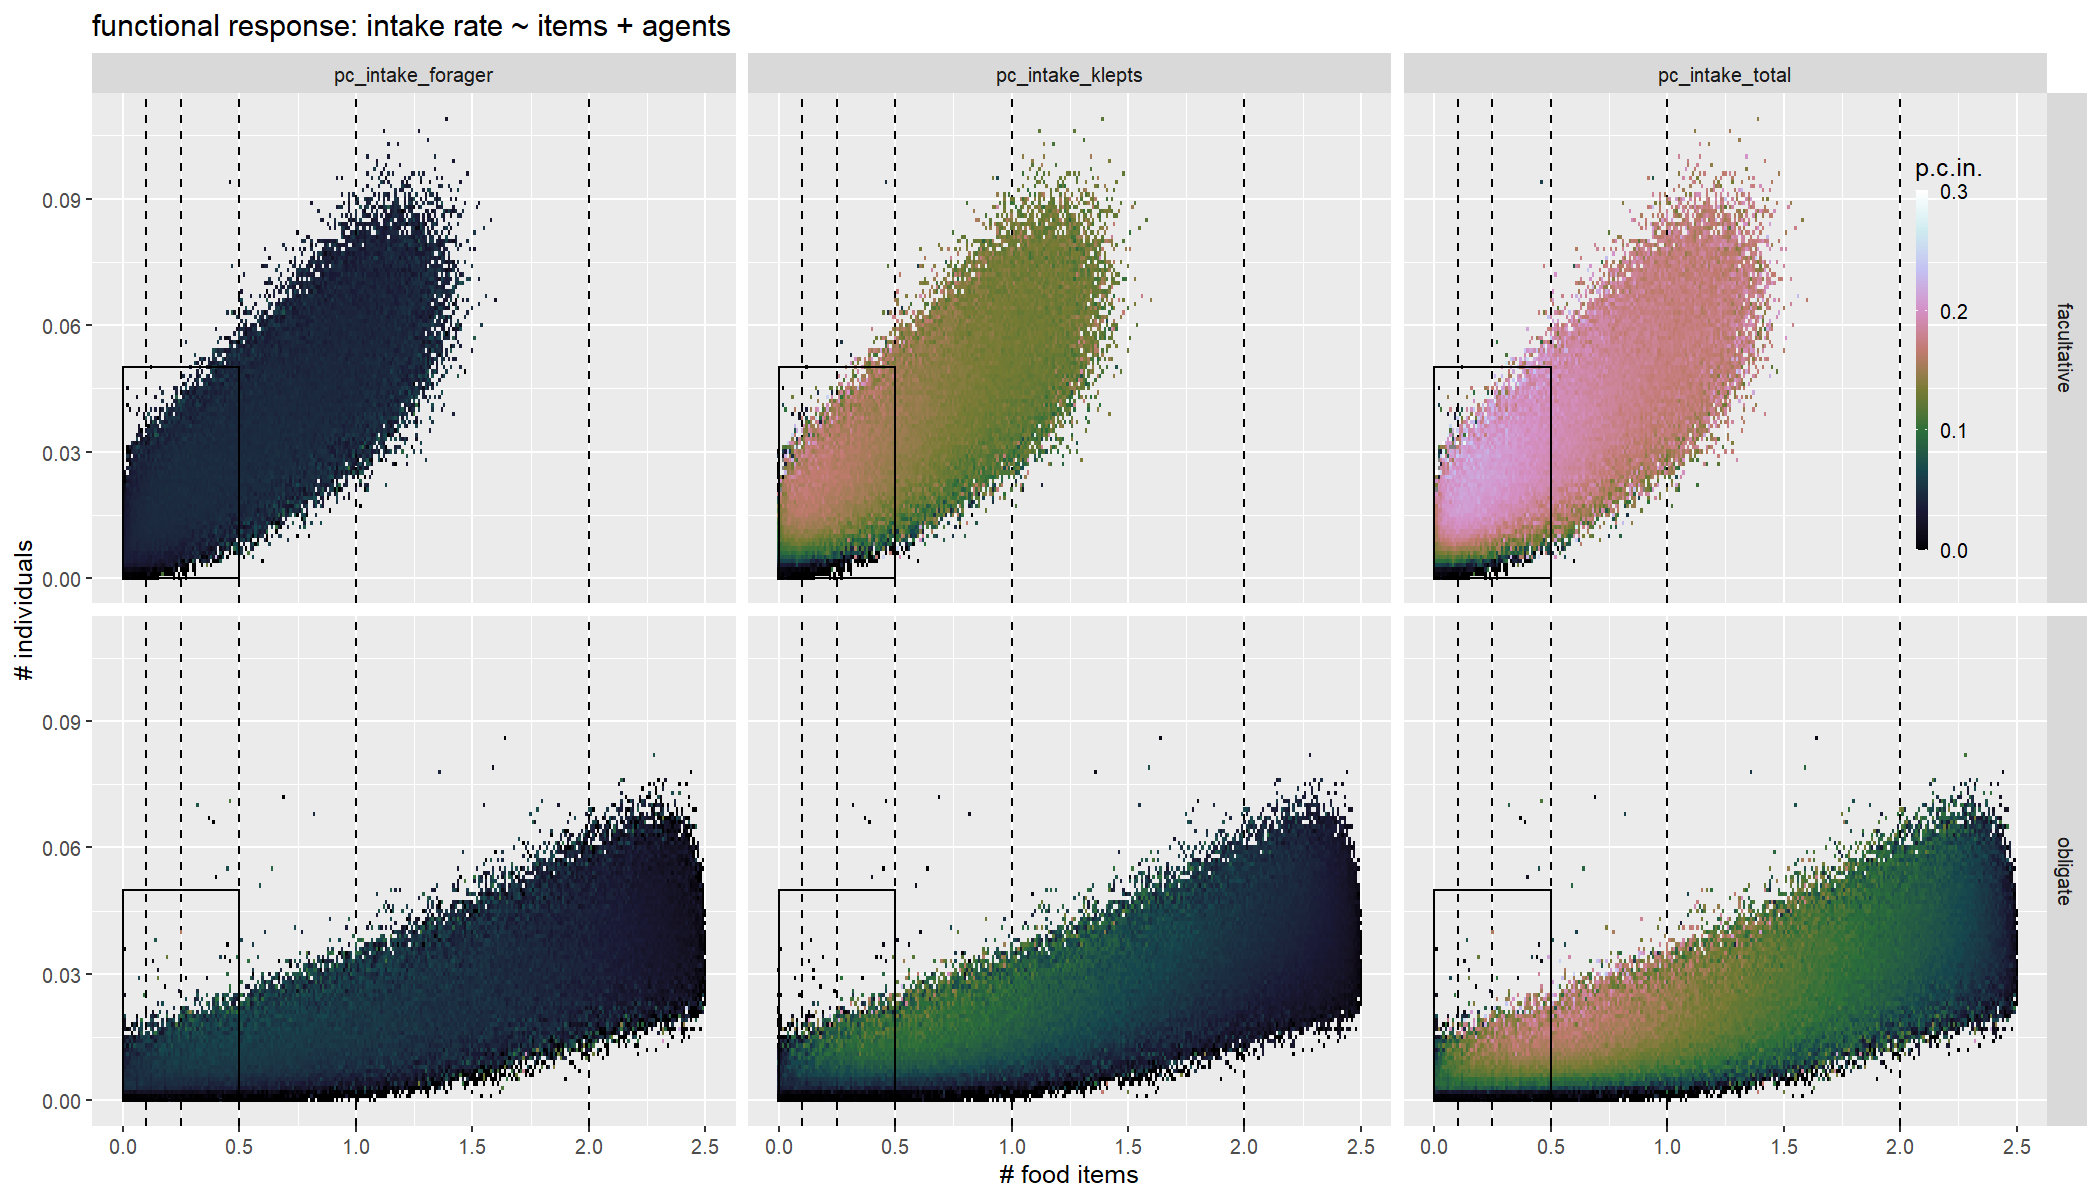
\includegraphics[width=0.60\textwidth]{figures/fig_fun_response_general.png}
% \caption{Figure legends can be longer than the titles of tables. However, they should not be excessively long.}
% \label{Fig:OkapiHorn}
% \end{figure}


%%%%%%%%%%%%%%%%%%%%%
% Videos
%%%%%%%%%%%%%%%%%%%%%
% If you have videos, journal style for them is similar to that for
% figures. You'll want to include a still image (such as a JPEG)
% to give your readers a preview of what the video looks like.

%%%%% Include the text below if you have videos

\renewcommand{\figurename}{Video} 
\setcounter{figure}{0}
% Thanks to Flo Debarre for the pro tip of putting
% \renewcommand{\figurename}{Video} before the Video legend and
% \renewcommand{\figurename}{Figure} after it!

% \begin{figure}[h!]
% %\includegraphics{VideoScreengrab.jpg}
% \caption{Video legends can follow the same principles as figure legends. Counters should be set and reset so that videos and figures are enumerated separately.}
% \label{VideoExample}
% \end{figure}

\renewcommand{\figurename}{Figure}
\setcounter{figure}{1}

%%%%% Include the above if you have videos


% \begin{figure}[h!]
% %\includegraphics{elegance}
% \caption{In this way, figure legends can be listed at the end of the document, with references that work, even though the graphic itself should be included for final files after acceptance. Instead, upload the relevant figure files separately to Editorial Manager; Editorial Manager should insert them at the end of the PDF automatically.}
% \label{Fig:AnotherFigure}
% \end{figure}

\subsection*{Online figure legends}

\renewcommand{\thefigure}{A\arabic{figure}}
\setcounter{figure}{0}

% \begin{figure}[h!]
% %\includegraphics{jumps20m}
% \caption{\textit{A}, the quick red fox proceeding to jump 20~m straight into the air over not one, but several lazy dogs. \textit{B}, the quick red fox landing gracefully despite the skepticism of naysayers.}
% \label{Fig:Jumps}
% \end{figure}

% \begin{figure}[h!]
% %\includegraphics{jumps20m}
% \caption{The quicker the red fox jumps, the likelier it is to land near an okapi. For further details, see \citet{LemKapEx07}.}
% \label{Fig:JumpsOk}
% \end{figure}

\renewcommand{\thefigure}{B\arabic{figure}}
\setcounter{figure}{0}

\end{document}
